\documentclass{beamer}
\mode<presentation>
\usetheme{CambridgeUS}
\usepackage[english, russian]{babel}
\usepackage[utf8]{inputenc}
\usepackage[T2A]{fontenc}
\usepackage{sansmathaccent}
\usepackage{alltt}
\linespread{0.8}
\usepackage{minted}

%\pdfmapfile{+sansmathaccent.map}
\title[C++]{Структуры данных}
\author{Наумов Д.А., доц. каф. КТ}
\date[11.10.2021] {Алгоритмы и структуры данных, 2021}

\begin{document}

%ТИТУЛЬНЫЙ СЛАЙД
\begin{frame}
  \titlepage
\end{frame}
  
%СОДЕРЖАНИЕ ЛЕКЦИИ
\begin{frame}
  \frametitle{Содержание лекции}
  \tableofcontents  
\end{frame}

\begin{frame}[fragile]{Массивы}
	\begin{itemize}
		\item статические
		\item динамические - массив, размер которого можно изменять в
процессе выполнения программы. 		
	\end{itemize}
	
~
	
\begin{minted}{c}
    //пример статического массива
    int array[n];
    
    //пример динамического массива vector
    vector<int> v;
    v.push_back(3); // [3]
    v.push_back(2); // [3,2]
    v.push_back(5); // [3,2,5]    
\end{minted}
\end{frame}

\begin{frame}[fragile]{Массивы}
	Доступ к элементам осуществляется так же, как в обычном массиве:
	\begin{minted}{c}
    cout << v[0] << "\n"; // 3
    cout << v[1] << "\n"; // 2
    cout << v[2] << "\n"; // 5
	\end{minted}
	
	~
	
	Еще один способ создать вектор – перечислить все его элементы:
	\begin{minted}{c}
    vector<int> v = {2,4,2,5,1};	
	\end{minted}	

    ~
    
	Можно также задать число элементов и их начальное значение:
	\begin{minted}{c}
    vector<int> a(8); // размер 8, начальное значение 0
    vector<int> b(8,2); // размер 8, начальное значение 2
	\end{minted}
\end{frame}

\begin{frame}[fragile]{Массивы}
    Функция \textit{size} возвращает число элементов вектора. В следующем коде мы обходим вектор и печатаем его элементы:

	\begin{minted}{c}
    for (int i = 0; i < v.size(); i++) {
        cout << v[i] << "\n";
    }
	\end{minted}
	
	~
	
	Обход вектора можно записать и короче:
	\begin{minted}{c}
    for (auto x : v) {
        cout << x << "\n";
    }
	\end{minted}
\end{frame}

\begin{frame}[fragile]{Массивы}
    Функция \textbf{back} возвращает последний элемент вектора, а функция \textbf{pop\_back} удаляет последний элемент:
	\begin{minted}{c}
    vector<int> v = {2,4,2,5,1};
    
    cout << v.back() << "\n"; // 1
    v.pop_back();
    cout << v.back() << "\n"; // 5
	\end{minted}

    ~

    Векторы реализованы так, что функции \textit{push\_back} и \textit{pop\_back} в среднем имеют сложность $O(1)$. 
    
    ~
    
    На практике работать с вектором почти так же быстро, как с массивом.
\end{frame}

\begin{frame}[fragile]{Итераторы}
    \textbf{Итератором} называется переменная, которая указывает на элемент структуры данных. 

    ~

    Итератор \textit{begin} указывает на первый элемент структуры, а итератор end -- на позицию за последним элементом. 

    ~

    Например, в случае вектора \textbf{v}, состоящего из восьми элементов, ситуация может выглядеть так:

	\begin{figure}[h]
		\centering
		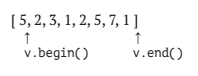
\includegraphics[scale=1.0]{images/lec11-pic01.png}
		%\caption{Пример таблицы цен отрезков стержня}
	\end{figure}

    ~
    
    Обратите внимание на асимметрию итераторов: 
	\begin{itemize}
		\item begin() указывает на элемент, принадлежащий структуре данных, 
		\item end() ведет за пределы структуры данных.	
	\end{itemize}
\end{frame}

\begin{frame}[fragile]{Диапазон}
    \textbf{Диапазоном} называется последовательность соседних элементов структуры данных. 
    
    ~
    
    Чаще всего диапазон задается с помощью двух итераторов:
    \begin{itemize}
        \item указывающего на первый элемент.
        \item указывающего на позицию за последним элементом.
    \end{itemize}

    В частности, итераторы \textit{begin()} и \textit{end()} определяют диапазон, содержащий все элементы структуры данных.

    ~
    
    Функции из стандартной библиотеки C++ обычно применяются к диапазонам. В следующем фрагменте сначала вектор сортируется, затем порядок его элементов меняется на противоположный, и, наконец, элементы перемешиваются в случайном порядке.

	\begin{minted}{c}
    sort(v.begin(),v.end());
    reverse(v.begin(),v.end());
    random_shuffle(v.begin(),v.end());
	\end{minted}
\end{frame}

\begin{frame}[fragile]{Диапазон}
    К элементу, на который указывает итератор, можно обратиться, воспользовавшись оператором *. В следующем коде печатается первый элемент вектора:
    \begin{minted}{c}
    cout << *v.begin() << "\n";
    \end{minted}
    
    ~
    Более полезный пример: функция \textbf{lower\_bound} возвращает итератор на
первый элемент отсортированного диапазона, значение которого не меньше $x$, а функция \textbf{upper\_bound} -- итератор на первый элемент, значение которого не больше $x$:

    \begin{minted}{c}
    vector<int> v = {2,3,3,5,7,8,8,8};
    
    auto a = lower_bound(v.begin(),v.end(),5);
    auto b = upper_bound(v.begin(),v.end(),5);

    cout << *a << " " << *b << "\n"; // 5 7
    \end{minted}

    В них применяется двоичный поиск, так что для поиска запрошенного элемента требуется логарифмическое время. Если искомый элемент не найден, то функция возвращает итератор на позицию, следующую за последним элементом диапазона.
\end{frame}

\begin{frame}[fragile]{Диапазон}
    В стандартной библиотеке C++ много полезных функций, заслуживающих внимания. 
    
    ~
    
    Например, в следующем фрагменте создается вектор, содержащий уникальные элементы исходного вектора в отсортированном порядке:
    
    \begin{minted}{c}
    sort(v.begin(),v.end());
    v.erase(unique(v.begin(),v.end()),v.end());
    \end{minted}
\end{frame}

\begin{frame}[fragile]{Двусторонняя очередь}
    \textbf{Двусторонней очередью (деком) }называется динамический массив, допускающий эффективные операции с обеих сторон. 
    
    ~
    
    Как и вектор, двусторонняя очередь предоставляет функции \textbf{push\_back} и \textbf{pop\_back}, но вдобавок к ним функции \textbf{push\_front} и \textbf{pop\_front}. 
    
    ~
    
    Пример использования:
    \begin{minted}{c}
    deque<int> d;
    
    d.push_back(5); // [5]
    d.push_back(2); // [5,2]
    d.push_front(3); // [3,5,2]
    d.pop_back(); // [3,5]
    d.pop_front(); // [5]
    \end{minted}
    
    Операции двусторонней очереди в среднем имеют сложность $O(1)$. 

    Однако постоянные множители для них больше, чем для вектора, поэтому использовать двусторонние очереди имеет смысл, только когда требуется выполнять какие­то действия на обеих сторонах структуры.
\end{frame}

\begin{frame}[fragile]{Стек}
    C++ предоставляет также специализированные структуры данных, по умолчанию основанные на двусторонней очереди. 
    
    ~
    
    Для стека определены функции \textbf{push} и \textbf{pop}, позволяющие вставлять и удалять элементы в конце структуры, а также функция \textbf{top}, возвращающая последний элемент без удаления:
    
    \begin{minted}{c}
    stack<int> s;
    
    s.push(2); // [2]
    s.push(5); // [2,5]
    
    cout << s.top() << "\n"; // 5
    
    s.pop(); // [2]
    
    cout << s.top() << "\n"; // 2
    \end{minted}
\end{frame}

\begin{frame}[fragile]{Очередь}
    В случае \textbf{очереди} элементы вставляются в начало, а удаляются из конца.
    
    ~
    
    Для доступа к первому и последнему элементам служат функции \textbf{front} и \textbf{back}.
    
    \begin{minted}{c}
    queue<int> q;
    
    q.push(2); // [2]
    q.push(5); // [2,5]
    
    cout << q.front() << "\n"; // 2
    
    q.pop(); // [5]
    
    cout << q.back() << "\n"; // 5
    \end{minted}
\end{frame}

\begin{frame}[fragile]{Множества}
    \textbf{Множеством} называется структура данных, в которой хранится набор элементов. Основные операции над множествами:
    \begin{itemize}
        \item вставка, 
        \item поиск
        \item удаление.
    \end{itemize}
    
    ~
    
    Множества реализованы так, что все эти операции эффективны, что часто позволяет улучшить время работы алгоритмов, в которых множества используются.

    ~
    
    В стандартной библиотеке C++ имеются две структуры, относящиеся к множествам:
    \begin{itemize}
        \item \textbf{set} основана на сбалансированном двоичном дереве поиска, его операции работают за время $O(log n)$, 
        \item \textbf{unordered\_set} основана на хеш­таблице и работает в среднем $O(1)$.
    \end{itemize}

    Обе структуры эффективны, и во многих случаях годится любая. Поскольку используются они одинаково, в примерах мы ограничимся только структурой \textit{set}.
\end{frame}

\begin{frame}[fragile]{Множества}
    В показанном ниже коде создается множество, содержащее целые числа, и демонстрируются некоторые его операции. 
    \begin{itemize}
        \item функция \textbf{insert} добавляет элемент во множество; 
        \item функция \textbf{count} возвращает количество вхождений элемента во множество;
        \item функция \textbf{erase} удаляет элемент из множества.
    \end{itemize}
    
    \begin{minted}{c}
    set<int> s;
    
    s.insert(3);
    s.insert(2);
    s.insert(5);
    
    cout << s.count(3) << "\n"; // 1
    cout << s.count(4) << "\n"; // 0
    
    s.erase(3);
    s.insert(4);
    
    cout << s.count(3) << "\n"; // 0
    cout << s.count(4) << "\n"; // 1
    \end{minted}
\end{frame}

\begin{frame}[fragile]{Множества}
    Важным свойством множеств является тот факт, что все их элементы различны. Следовательно, функция \textbf{count} всегда возвращает 0 (если элемент не принадлежит множеству) или 1 (если принадлежит), а функция insert никогда не добавляет элемент во множество, если он в нем уже присутствует. Это демонстрируется в следующем фрагменте:

    \begin{minted}{c}
    set<int> s;
    
    s.insert(3);
    s.insert(3);
    s.insert(3);
    
    cout << s.count(3) << "\n"; // 1
    \end{minted}
\end{frame}

\begin{frame}[fragile]{Множества}
    Множество в основном можно использовать как вектор, однако доступ к элементам с помощью оператора [] невозможен. В следующем коде печатается количество элементов во множестве, а затем эти элементы перебираются:
    \begin{minted}{c}
    cout << s.size() << "\n";
    
    for (auto x : s) {
        cout << x << "\n";
    }
    \end{minted}
\end{frame}

\begin{frame}[fragile]{Множества}
    Функция \textbf{find(x)} возвращает итератор, указывающий на элемент со значением $x$. Если же множество не содержит $x$, то возвращается итератор \textit{end()}.

    \begin{minted}{c}
    auto it = s.find(x);

    if (it == s.end()) {
	    // x не найден
    }
    \end{minted}
\end{frame}

\begin{frame}[fragile]{Упорядоченные множества}
    Основное различие между двумя структурами множества в C++ – то, что \textbf{set} упорядочено, а \textbf{unordered\_set} не упорядочено. Поэтому если порядок элементов важен, то следует пользоваться структурой \textit{set}.

    ~
    
    Рассмотрим задачу о нахождении наименьшего и наибольшего значений во множестве. Чтобы сделать это эффективно, необходимо использовать структуру \textit{set}.
    
    ~
    
    Поскольку элементы отсортированы, найти наименьшее и наибольшее значения можно следующим образом:
    \begin{minted}{c}
    auto first = s.begin();
    auto last = s.end(); last--;
    
    cout << *first << " " << *last << "\n";
    \end{minted}
    
    Отметим, что поскольку \textit{end()} указывает на позицию, следующую за последним элементом, то необходимо уменьшить итератор на единицу.
\end{frame}

\begin{frame}[fragile]{Упорядоченные множества}
    В структуре \textbf{set} имеются также функции \textbf{lower\_bound(x)} и \textbf{upper\_bound(x)}, которые возвращают итератор на наименьший элемент множества, значение которого не меньше x или больше x соответственно. Если искомого элемента не существует, то обе функции возвращают \textbf{end()}.
    
    \begin{minted}{c}
    cout << *s.lower_bound(x) << "\n";
    cout << *s.upper_bound(x) << "\n";
    \end{minted}
\end{frame}

\begin{frame}[fragile]{Мультимножества}
    В отличие от множества, в \textbf{мультимножество} один и тот же элемент может входить несколько раз. 
    
    ~
    
    В C++ имеются структуры \textbf{multiset} и \textbf{unordered\_multiset}, похожие на \textbf{set} и \textbf{unordered_set}. 
    
    ~
    
    В следующем коде в мультимножество три раза добавляется значение 5.
    \begin{minted}{c}
    multiset<int> s;
    
    s.insert(5);
    s.insert(5);
    s.insert(5);
    
    cout << s.count(5) << "\n"; // 3
    \end{minted}
\end{frame}

\begin{frame}[fragile]{Мультимножества}    
    Функция \textbf{erase} удаляет все копии значения из мультимножества.
    
    \begin{minted}{c}
    s.erase(5);

    cout << s.count(5) << "\n"; // 0
    \end{minted}
    
    Если требуется удалить только одно значение, то можно поступить так:
    \begin{minted}{c}
    s.erase(s.find(5));
    
    cout << s.count(5) << "\n"; // 2
    \end{minted}
    
    ~
    
    Отметим, что во временной сложности функций \textbf{count} и \textbf{erase} имеется дополнительный множитель $O(k)$, где $k$ -– количество подсчитываемых (удаляемых) элементов. В частности, подсчитывать количество копий значения в мультимножестве с помощью функции count неэффективно.
\end{frame}

\begin{frame}[fragile]{Отображения}
    \textbf{Отображением} называется множество, состоящее из пар ключ-значение. Отображение можно также рассматривать как обобщение массива.
    
    ~
    
    Если в обыкновенном массиве ключами служат последовательные целые числа 0, 1,..., $n−1$, где n – размер массива, то в отображении ключи могут иметь любой тип и необязательно должны быть последовательными.
    
    ~
    
    В стандартной библиотеке C++ есть две структуры отображений, соответствующие структурам множеств: в основе map лежит сбалансированное двоичное дерево со временем доступа к элементам $O(log n)$, а в основе \textbf{unordered\_map} – техника хеширования со средним временем доступа к элементам O(1).
\end{frame}

\begin{frame}[fragile]{Отображения}
    В следующем фрагменте создается отображение, ключами которого являются строки, а значениями – целые числа:
    \begin{minted}{c}
    map<string,int> m;
    
    m["monkey"] = 4;
    m["banana"] = 3;
    m["harpsichord"] = 9;
    
    cout << m["banana"] << "\n"; // 3
    \end{minted}
    
    Если в отображении нет запрошенного ключа, то он автоматически добавляется, и ему сопоставляется значение по умолчанию. Например, в следующем коде в отображение добавляется ключ «aybabtu» со значением 0.
    \begin{minted}{c}
    map<string,int> m;
    
    cout << m["aybabtu"] << "\n"; // 0
    \end{minted}
\end{frame}

\begin{frame}[fragile]{Отображения}
    Функция \textbf{count} проверяет, существует ли ключ в отображении. 
    \begin{minted}{c}
    if (m.count("aybabtu")) {
        //ключ "aybabtu" есть в отображении
    }
    \end{minted}
    
    ~
    
    В следующем коде печатаются все имеющиеся в отображении ключи и
значения:
    \begin{minted}{c}
    for (auto x : m) {
        cout << x.first << " " << x.second << "\n";
    }
    \end{minted}
\end{frame}

\begin{frame}[fragile]{Очереди с приоритетом}
    \textbf{Очередь с приоритетом} -- это мультимножество, которое поддерживает вставку, а также извлечение и удаление минимального или максимального элемента (в зависимости от типа очереди). Вставка и удаление занимают время $O(log n)$, а извлечение – время $O(1)$.
    
    ~
    
    Очередь с приоритетом обычно основана на структуре пирамиды (\textbf{heap}), представляющей собой двоичное дерево специального вида. Структура \textbf{multiset} и так предоставляет все операции, которые определены в очереди с приоритетом, и даже больше, но у очереди с приоритетом есть достоинство -- меньшие постоянные множители в оценке временной сложности.
    
    ~
    
    Поэтому если требуется только найти минимальный или максимальный элемент, то лучше использовать очередь с приоритетом, а не множество или мультимножество.
\end{frame}

\begin{frame}[fragile]{Очереди с приоритетом}
    По умолчанию элементы очереди с приоритетом в C++ отсортированы в порядке убывания, так что поддерживаются поиск и удаление наибольшего элемента, что и продемонстрировано в следующем коде:

    \begin{minted}{c}
    priority_queue<int> q;
    
    q.push(3);
    q.push(5);
    q.push(7);
    q.push(2);
    cout << q.top() << "\n"; // 7

    q.pop();
    cout << q.top() << "\n"; // 5
    
    q.pop();
    q.push(6);
    cout << q.top() << "\n"; // 6
    q.pop();
    \end{minted}
\end{frame}

\begin{frame}[fragile]{Множества, основанные на политиках}
    Компилятор g++ предоставляет также несколько структур данных, не входящих в стандартную библиотеку C++. Они называются \textbf{структурами, основанными на политиках} (policy based structure). 
    
    ~
    
    Для их использования в программу нужно включить такие строки:
    \begin{minted}{c}
    #include <ext/pb_ds/assoc_container.hpp>
    
    using namespace __gnu_pbds;
    \end{minted}

    ~
    
    После этого можно определить структуру данных \textbf{indexed\_set}, которая похожа на множество, но допускает индексирование как массив. Для значений типа \textit{int} определение выглядит так:
    \begin{minted}{c}
    typedef tree <int, null_type, less<int>, rb_tree_tag,
        tree_order_statistics_node_update> indexed_set;
    \end{minted}
    \end{frame}

\begin{frame}[fragile]{Множества, основанные на политиках}
    А создается множество так:
    
    \begin{minted}{c}
    indexed_set s;
    
    s.insert(2);
    s.insert(3);
    s.insert(7);
    s.insert(9);
    \end{minted}
    
    
    Особенность этого множества состоит в том, что доступ можно осуществлять по индексу, который элемент имел бы в отсортированном массиве.
    
    ~
    
    Функция \textbf{find\_by\_order} возвращает итератор, указывающий на элемент в заданной позиции:
    
    \begin{minted}{c}
    auto x = s.find_by_order(2);
    cout << *x << "\n"; // 7
    \end{minted}
    
\end{frame}

\begin{frame}[fragile]{Множества, основанные на политиках}    
    Функция order\_of\_key возвращает позицию заданного элемента:
    \begin{minted}{c}
    cout << s.order_of_key(7) << "\n"; // 2
    \end{minted}
    
    Если элемент отсутствует во множестве, то мы получим позицию, в которой он находился бы, если бы присутствовал:
    \begin{minted}{c}
    cout << s.order_of_key(6) << "\n"; // 2
    cout << s.order_of_key(8) << "\n"; // 3
    \end{minted}
    Время работы обеих функций логарифмическое.
\end{frame}


\begin{frame}[fragile]{Эксперименты}
    Приведем некоторые результаты, касающиеся практической эффективности описанных выше структур данных. 
    
    ~
    
    Хотя временная сложность -- отличный инструмент, она не всегда сообщает всю правду об эффективности, поэтому имеет смысл провести эксперименты с настоящими реализациями и наборами данных.

    ~
    
    Многие задачи можно решить, применяя как множества, так и сортировку. Важно понимать, что алгоритмы на основе сортировки обычно гораздо быстрее, даже если это не очевидно из одного лишь анализа временной сложности
\end{frame}

\begin{frame}[fragile]{Эксперименты}
    В качестве примера рассмотрим \textbf{задачу о вычислении количества уникальных элементов вектора}. 
    
    ~
    
    \begin{itemize}
        \item Одно из возможных решений – поместить все элементы во множество и вернуть размер этого множества. Поскольку порядок элементов не важен, можно использовать как \textit{set}, так и \textit{unordered\_set}. 
        \item  Можно решить задачу и по­другому: сначала отсортировать вектор, а затем обойти его элементы. Подсчитать количество уникальных элементов отсортированного вектора просто.
    \end{itemize}
    
\end{frame}

\begin{frame}[fragile]{Эксперименты}
    В табл. приведены результаты эксперимента, в котором оба алгоритма тестировались на случайных векторах чисел типа \textit{int}. 
    
	\begin{figure}[h]
		\centering
		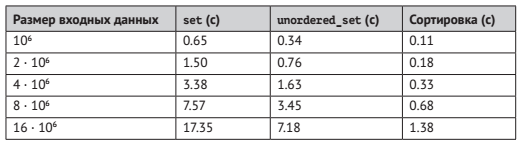
\includegraphics[scale=0.75]{images/lec11-pic02.png}
		%\caption{Пример таблицы цен отрезков стержня}
	\end{figure}

    \begin{itemize}
        \item Оказалось, что алгоритм на основе \textit{unordered\_set} примерно в два раза быстрее алгоритма на основе \textit{set}, а алгоритм на основе сортировки быстрее алгоритма на основе \textit{set} более чем в 10 раз.
        \item Отметим, что временная сложность обоих алгоритмов равна $O(n log n)$, и тем не менее алгоритм на основе сортировки работает гораздо быстрее. 
        \item Причина в том, что сортировка -- простая операция, тогда как сбалансированное двоичное дерево поиска, применяемое в реализации set, – сложная структура данных.
    \end{itemize}
    
\end{frame}

\begin{frame}[fragile]{Сравнение отображения и массива}
    \textbf{Отображения} -– удобные структуры данных, по сравнению с массивами, поскольку позволяют использовать индексы любого типа, но и постоянные множители велики. 

    ~
    
    В следующем эксперименте мы создали вектор, содержащий $n$ случайных целых чисел от 1 до 106, а затем искали самое часто встречающееся значение путем подсчета числа вхождений каждого элемента. 
    
    ~
    
    Сначала мы использовали отображения, но поскольку число 106 достаточно мало, то можно использовать и массивы.
\end{frame}

\begin{frame}[fragile]{Сравнение отображения и массива}
    Результаты эксперимента сведены в табл. 
    
    \begin{figure}[h]
		\centering
		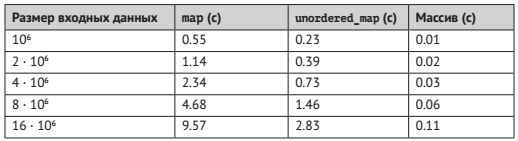
\includegraphics[scale=0.75]{images/lec11-pic03.png}
		%\caption{Пример таблицы цен отрезков стержня}
	\end{figure}

    Хотя \textit{unordered\_map} примерно в три раза быстрее \textit{map}, массив все равно почти в 100 раз быстрее.
    
    ~
    
    Таким образом, по возможности следует пользоваться массивами, а не отображениями. Особо отметим, что хотя временная сложность операций \textit{unordered\_map} равна O(1), скрытые постоянные множители, характерные для этой структуры данных, довольно велики.
\end{frame}

\begin{frame}[fragile]{Сравнение очереди с приоритетом и мультимножества}
    Верно ли, что очереди с приоритетом действительно быстрее мультимножеств? Чтобы выяснить это, мы провели еще один эксперимент. 
    
    ~
    
    Мы создали два вектора, содержащие $n$ случайных чисел типа $int$. Сначала мы добавили все элементы первого вектора в структуру данных, а затем обошли второй вектор и на каждом шаге удаляли наименьший элемент из структуры данных и добавляли в нее новый элемент.
\end{frame}

\begin{frame}[fragile]{Сравнение очереди с приоритетом и мультимножества}
    Результаты эксперимента представлены в табл.
    
    \begin{figure}[h]
		\centering
		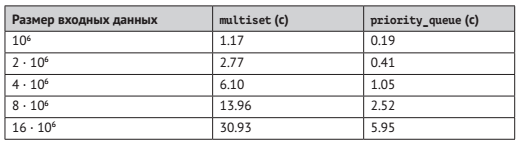
\includegraphics[scale=0.75]{images/lec11-pic04.png}
		%\caption{Пример таблицы цен отрезков стержня}
	\end{figure}

    Оказалось, что с помощью очереди с приоритетом эта задача решается примерно в пять раз быстрее, чем с помощью мультимножества.
\end{frame}

\end{document}